%%% License: Creative Commons Attribution Share Alike 4.0 (see https://creativecommons.org/licenses/by-sa/4.0/)
%%% Slides are based heavily on earlier versions of this course taught by Jesper Rudiger.

\documentclass[english,10pt
%,handout
,aspectratio=169
]{beamer}
%%% License: Creative Commons Attribution Share Alike 4.0 (see https://creativecommons.org/licenses/by-sa/4.0/)
%%% Slides are based heavily on earlier versions of this course taught by Jesper Rudiger and Peter Norman Sorensen.

\DeclareGraphicsExtensions{.eps, .pdf,.png,.jpg,.mps,}
\usetheme{reMedian}
\usepackage{parskip}
\makeatother

\renewcommand{\baselinestretch}{1.1} 

\usepackage{amsmath, amssymb, amsfonts, amsthm}
\usepackage{enumerate}
\usepackage{hyperref}
\usepackage{url}
\usepackage{bbm}
\usepackage{color}

\usepackage{tikz}
\usepackage{tikzscale}
\newcommand*\circled[1]{\tikz[baseline=(char.base)]{
		\node[shape=circle,draw, inner sep=-20pt] (char) {#1};}}
\usetikzlibrary{automata,positioning}
\usetikzlibrary{decorations.pathreplacing}
\usepackage{pgfplots}
\usepgfplotslibrary{fillbetween}
\usepackage{graphicx}

\usepackage{setspace}
%\thinmuskip=1mu
%\medmuskip=1mu 
%\thickmuskip=1mu 


\usecolortheme{default}
\usepackage{verbatim}
\usepackage[normalem]{ulem}

\usepackage{apptools}
\AtAppendix{
	\setbeamertemplate{frame numbering}[none]
}
\usepackage{natbib}



\title{Financial Markets Microstructure \\ Lectures 17 \& 18}

\subtitle{Algo-trading, High-Frequency Trading, and Blockchain}

\author{Egor Starkov}

\date{K{\o}benhavns Unversitet \\
	Spring 2021}


\begin{document}
	\AtBeginSection[]{
		\frame<beamer>{
			\frametitle{This lecture:}
			\tableofcontents[currentsection,currentsubsection]
	}}
	\frame[plain]{\titlepage}


\begin{frame}{Previously on FMM}
	\textbf{Corporate governance} has a lot of connection to company's financial market performance
	\begin{itemize}
		\item access to capital affected by liq-ty
		\item liq-ty and corporate control are somewhat antithetical
		\item firm can use stock price as market's feedback on its decisions or as benchmark of CEO performance
		\item firms have some ways in which they can improve the liquidity of their stocks
	\end{itemize}
\end{frame}


\begin{frame}{Today on FMM...}
	\begin{itemize}
		\item Algo-trading!
		\item High-frequency trading!
		\item Cryptocurrencies!
		\item and more...
	\end{itemize}
\end{frame}


%\begin{frame}{Going forward}
%	A method for reading research articles (esp. theoretical ones)
%	\begin{enumerate}
%		\item Read abstract and introduction
%		\item Browse through the rest
%		\item Read model and results in detail
%		\item Read conclusion, and re-read abstract and introduction
%	\end{enumerate}
%	(Does not apply to surveys -- those are readable as usual.)
%\end{frame}


\begin{frame}{Digital Markets}
	\begin{quotation}
		``...It should come as no surprise then that the financial system exhibits a Moore's Law of its own -- from 1929 to 2009 the total \structure{market capitalization} of the US stock market has \structure{doubled every decade}. The total \alert{trading volume} of stocks in the Dow Jones Industrial Average \alert{doubled every 7.5 years} during this period, but in the most recent decade, the \alert{pace has accelerated}: now the doubling occurs every 2.9 years, growing almost as fast as the semiconductor industry.''
		\begin{flushright}
			\cite{kirilenko_moores_2013}
		\end{flushright}
	\end{quotation}
\end{frame}


\begin{frame}{Digital Markets}
	\begin{columns}
		\begin{column}{0.6\linewidth}
			{\setstretch{1.3}
				\begin{itemize}
					\item The digital revolution of the past few decades has reshaped financial markets as much as (if not more than) any other aspect of our lives
					\item The quote above mentions the \structure<1>{``extensive margin''} akin to the Moore's Law
					\item But the \structure<2>{``intensive margin''} is also at work
					\pause
					\begin{itemize}
						\item Index funds, automated arbitrage, automated execution \& market-making only made possible by computers
					\end{itemize}
					\pause
					\item In addition to Moore's Law, \structure<3>{Murphy's Law} does not fail either
					\begin{itemize}
						\item If something can go wrong it will, and the scope for failures is as big as ever these days. See \cite{kirilenko_moores_2013} (pp.60-67) for five stories.
					\end{itemize}
				\end{itemize}
			}
		\end{column}
		\begin{column}{0.4\linewidth}
			\pause[1]
			\includegraphics<handout:0>[width=\linewidth]{pics/mainframe}
		\end{column}
	\end{columns}
\end{frame}



\section{Algo-trading: Some numbers}

\begin{frame}{More on algo-trading}
	\begin{itemize}
		\item Algorithms allow for a lot of stuff:
		\begin{itemize}
			\item \structure{HFT} (later today)
			\item better \structure{hedging} though some automated hedges
			\item but also for better \alert{execution} via order-splitting.
		\end{itemize}
		\item \cite{beason_anatomy_2019} give some (actually a lot of) info on how algorithms work for large \structure{institutional investors} (a typical counterpart to HFT nowadays)
		\item ``Parent'' orders are split (by algorithms) into many ``child'' orders that are routed to markets
	\end{itemize}
\end{frame}


\begin{frame}{Institutional algo-trading}
	\begin{itemize}
		\item The average parent order attempts to trade \$287,000 over 84
		minutes, equivalent to 4.80 percent of volume over the duration of the order.
		\pause[3]
		\begin{itemize}
			\item avg: 63.1 runs per parent (avg 10m total duration), 8.8 children per run
		\end{itemize}
		\pause[2]
		\only<2-3|handout:0>{
			\item \alert{Bliz Quiz:} how many child orders do you think every parent order spawns?
			\begin{enumerate}
				\item 5-10
				\item 20-50
				\item 100-200
				\item \structure<3>{400-800}
			\end{enumerate}
		}
		\only<4-5|handout:0>{
			\item \alert{Bliz Quiz:} how many of these child orders are market orders?
			\begin{enumerate}
				\item \structure<5>{$<1\%$}
				\item $5-10\%$
				\item $\approx 50\%$
				\item $>99\%$
			\end{enumerate}
		}
		\pause[5]
		\item Of the 300 million child orders, less than 0.40 percent are market orders.
		\pause[6]
		\begin{itemize}
			\item By comparison, retail investors usage of market orders is over 50 percent
			\item $\approx 80\%$ are limit orders, $\approx 20\%$ are PEG orders -- dark limit orders that are dynamically “pegged” to the NBBO
			\item Of the limit orders, $24\%$ are marketable, $65\%$ are passive, rest inside the spread
		\end{itemize}
		\item Many orders are unfilled (even marketable)
		\begin{itemize}
			\item Conditional on filled, median time-to-trade=5ms
			\item Even unfilled orders have price impact
		\end{itemize}
	\end{itemize}
\end{frame}



\section{HFT 1: Investment in speed}


\begin{frame}{High-frequency trading: introduction}
	\begin{itemize}
		\item \textbf{\href{https://static.fjcdn.com/gifs/Gotta+go+fast+an+animated+gif+i+made_caabed_4923630.gif}{HFT}}: Refers to computerized, algorithmic trading at high pace: fastest participants take advantage of opportunities before others
		\item \textbf{Speed is key}: for instance, in 2010, a USD 300 million cable was laid between Chicago and New Jersey (Nasdaq)
		\item \textbf{Ubiquitous}: estimated to account for more than 50\% of volume in the US and more than 25\% in Europe
		\item \textbf{Recent phenomenon(?)}: the effect on markets is still not well understood. Few empirical studies and fewer theoretical models
		%\item \textbf{Controversial}: all those market crashes I mentioned? 
		\item \textbf{Today}: Look at two models of HFT
	\end{itemize}
\end{frame}


\begin{frame}{\citet*{biais_equilibrium_2015}}
	\begin{columns}
		\begin{column}{0.6\linewidth}
			{\setstretch{1.3}
				\begin{itemize}
					\item Simple model of fast trading and \structure{investment in speed}
					\item Look at equilibrium behavior and welfare implications
					\item Endogenize the choice of whether to be fast or slow - optimal decision depends on size of trader
				\end{itemize}
			}
		\end{column}
		\begin{column}{0.4\linewidth}
			\pause[1]
			\includegraphics<handout:0>[width=\linewidth]{pics/hftrade}
		\end{column}
	\end{columns}

\end{frame}


\begin{frame}{Model: basics}
	\begin{itemize}
		\item \textbf{Institution}: continuum of profit-maximizing financial institutions indexed by $i$, zero endowment, trade one unit 
		\item \textbf{Time}: $\tau \in \{0,1,2\}$
		\item \textbf{Asset value}: $u_{i}=v+y_{i}$, where $v$ is the fundamental value and $y$ the institution's private value 
		\begin{itemize}
			\item \textbf{Fundamental value}: $v \in \{\mu-\epsilon, \mu + \epsilon\}$, equal probability, realized at $\tau=2$
			\item \textbf{Private value}: $y_{i} \in \{\delta, -\delta\}$, equal probability and i.i.d. across investors, observed at $\tau=1$ 
		\end{itemize}
		\item \textbf{Trading}: Occurs at $\tau=1$ after private values are learned
	\end{itemize}
\end{frame}


\begin{frame}{Model: high-frequency trading}
	\begin{itemize}
		\item \textbf{HFT}: A fraction $\alpha$ of the institutions invest at $\tau =0$ to become HFT
		\item \textbf{Information}: Let's call HFT \textit{fast} institutions (viz. \textit{slow} institutions)
		\begin{itemize}
			\item Fast institutions have better information: learn $v$ at $\tau=1$ whereas slow institutions learn $v$ at $\tau=2$
			\item Fast institutions find a trading opportunity with probability one, slow institutions with probability $\rho<1$
		\end{itemize}
		\item \textbf{Timing}
		\begin{enumerate}
			\item Each institution $i$ observes $y_{i}$, and if fast, observes $v$
			\item Each institution $i$ finds a trading opportunity or not. If yes, chooses whether to buy/sell/abstain
			\item Liquidity providers execute order $\omega$ at price $\mathbb{E}(v|\omega)$
			(implicit assumption of market maker competition)
		\end{enumerate}
	\end{itemize}
\end{frame}


\begin{frame}{Information}
	\begin{itemize}
		\item \textbf{Fundamental value:} Good news/bad news:
		\begin{itemize}
			\item \structure{Good news} refer to high value: $v=\mu+\epsilon$.
			\item \alert{Bad news} refer to low value: $v=\mu-\epsilon$.
		\end{itemize}
		\item \textbf{Fast institutions} (FI) have the following types
		\begin{itemize}
			\item $GH$: Good news, high private valuation
			\item $GL$: Good news, low private valuation
			\item $BH$: Bad news, high private valuation
			\item $BL$: Bad news, low private valuation
		\end{itemize}
		\item \textbf{Slow institutions} (SI), on the other hand, are either
		\begin{itemize}
			\item $H$: high private valuation
			\item $L$: low private valuation
		\end{itemize}
	\end{itemize}
\end{frame}


\begin{frame}{Equilibrium analysis}
	\begin{itemize}
		\item \textbf{No fast trading}: If $\alpha=0$ all orders execute at $\mu$
		\item \textbf{Active fast trading}: Now suppose $\alpha>0$. Let
		\smallskip
		\begin{center}
			$
			\displaystyle
			\begin{aligned}
			\beta^{F}_{j}: & \text{ prob. that fast institution type $j$ buys} \\ 
			\beta^{S}_{j}: & \text{ prob. that slow institution type $j$ buys (cond. on trading opp-ty)} 
			\end{aligned}
			$
		\end{center}
		\item \textbf{High value}: Fast $GH$ types have highest possible valuation: $\beta^{F}_{GH}=1$
		\item \textbf{Low value}: Fast $BL$ types have lowest possible valuation: $\beta^{G}_{BL}=0$
		\item \textbf{Buy side}: Let $a  =\mathbb{E}[v|buy]$. Use above observation and Bayes' Rule to get
		\[a =\mu+\frac{\alpha\frac{1+\beta^{F}_{GL}-\beta^{F}_{BH}}{4}}{(1-\alpha)\rho\frac{\beta^{S}_{H}+\beta^{S}_{L}}{2}+\alpha\frac{1+\beta^{F}_{GL}+\beta^{F}_{BH}}{4}} \epsilon.
		\]
	\end{itemize}
\end{frame}


\begin{frame}{Multiple equilibria}
	\begin{itemize}
		\item \textbf{Multiple equilibria}: Often markets have several equilibria.
		\item \textbf{Self-fulfilling expectations}: This is caused by the endogenous price:
		\begin{itemize}
			\item If you think buyers will have high valuations $\rightarrow$ set high $a$
			\item If $a$ is high, only traders with high valuations will buy
		\end{itemize}
		\item \textbf{Assumption}:  $\frac{\epsilon}{2} < \delta < \epsilon$: both $v$ and $y$ matter; $v$ more so.
		\item \textbf{Value ranking}: Let $V^i_j$ be the value of a type-$i$ institution with type-$j$ information. Then the assumption implies
		\[
		V^F_{GH}>V^S_H>V^F_{GL}>\mu>V^F_{BH}>V^S_L>V^F_{BL}.
		\]
		\item \textbf{Equilibrium types}: We focus here on the pure strategy equilibria. There will be three types of equilibria: P1, P2 and P3.
	\end{itemize}
\end{frame}


\begin{frame}{}
	\begin{itemize}
		\item \textbf{P1}: $\mu \leq a < \mu + \epsilon-\delta$. Fast institutions with good news always buy, slow institutions buy if private value high: 
		\[
		\beta^{F}_{GL}=\beta^{S}_{H}=1 \text{ and }\beta^{F}_{BH}=\beta^S_L=0
		\]
		\item \textbf{P2}: $\mu+\epsilon-\delta<a<\mu+\delta$. Fast institutions with good news and high value buy, but don't trade if information is conflicting. Slow institutions buy if private value high: 
		\[
		\beta^{F}_{GL}=\beta^S_L=\beta^{F}_{BH}=0 \text{ and }\beta^{S}_{H}=1
		\]
		\item \textbf{P3}: $a=\mu+\epsilon$. Fast institutions with good news and high value buy, other types of institutions don't trade (\textit{crowding out}):
		\[
		\beta^{F}_{GL}=\beta^{S}_{H}=\beta^{F}_{BH}=\beta^S_L=0
		\]
		\item Note: as usual, we look on one side of mkt so "sell" same as "abstain" in betas above
	\end{itemize}
\end{frame}


\begin{frame}{When do we have multiple equilibria?}
	\begin{itemize}
		\item \textbf{P3 equilibrium}: Always exists. If dealers believe only fast institutions trade $\rightarrow$  high $a$. But then only optimal for fast institutions to trade.
		\item \textbf{Proposition}: $P1$ equilibrium exists if $\alpha<\alpha_{P1} \equiv \frac{\rho(\epsilon-\delta)}{\rho(\epsilon-\delta)+\delta}$. Proof. 
		\begin{enumerate}
			\item Suppose institutions expect $a=\mu + \frac{\alpha}{\alpha+(1-\alpha)\rho} \epsilon$ 
			\item Notice $\mu-\epsilon+\delta<\mu<a$: FI never buy with bad news (\structure{$\beta^{F}_{BH}=0$ optimal})
			\item $\alpha<\alpha_{P1} \Rightarrow a<\mu+\epsilon-\delta$: good news imply expected FI gains from buying, regardless of private valuation
			(\structure{$\beta^{F}_{GL}=1$ is optimal}).
			\item Notice $\mu+\delta>\mu+\epsilon/2>\mu+\epsilon-\delta >a$: SI with high valuation always buys (\structure{$\beta^{S}_{H}=1$ is optimal}).
			\item Conditional on this, $\mathbb{E}[v|buy]=\mu + \frac{\alpha}{\alpha+(1-\alpha)\rho} \epsilon$ (\structure{$a$ is optimal price}). \qed
		\end{enumerate}
		\item Similarly, can find values of $\alpha$ s.t. $P2$ equilibrium exists
		\item $P1$ is Pareto dominant for $\alpha<\alpha_{P1}$. 
	\end{itemize}
\end{frame}


\begin{frame}{Institution gain (Fast Institutions)}
	\begin{itemize}
		\item FI gain in $P1$ equilibrium is (focus on buy side):
		\begin{align*}
		\mathbb{E}[u-a|buy, FI]
		& = \mathbb{E}[u|buy, FI] - \left[\mu + \frac{\alpha}{\alpha+(1-\alpha)\rho} \epsilon\right] \\
		& = \mathbb{E}[u|v=\mu+\epsilon] - \left[\mu + \frac{\alpha}{\alpha+(1-\alpha)\rho} \epsilon\right] \\
		& = \mu+\epsilon - \left[\mu + \frac{\alpha}{\alpha+(1-\alpha)\rho} \epsilon\right] \\
		& = \frac{(1-\alpha)\rho}{\alpha+(1-\alpha)\rho} \epsilon \equiv \phi(\alpha)
		\end{align*}
		\item Notice $\phi'(\alpha)<0$.
	\end{itemize}
\end{frame}


\begin{frame}{Institution gain (Slow Institutions)}
	\begin{itemize}
		\item SI gain in $P1$ equilibrium is (focus on buy side):
		\begin{align*}
		\mathbb{E}[u-a|buy, SI]
		& = \mathbb{E}[u|buy, SI] - \left[\mu + \frac{\alpha}{\alpha+(1-\alpha)\rho} \epsilon\right] \\
		& = \mathbb{E}[u|y_{i}=\delta] - \left[\mu + \frac{\alpha}{\alpha+(1-\alpha)\rho} \epsilon\right] \\
		& = \mu+\delta - \left[\mu + \frac{\alpha}{\alpha+(1-\alpha)\rho} \epsilon\right] \\
		& = \delta -  \frac{\alpha}{\alpha+(1-\alpha)\rho} \epsilon \equiv \psi(\alpha)
		\end{align*}
		\item Notice $\psi'(\alpha)<0$.
	\end{itemize}
\end{frame}


\begin{frame}{Institution gain}
	\begin{itemize}
		\item Both $\phi(\alpha)$ and $\psi(\alpha)$ are decreasing in $\alpha$: all trader types lose when proportion of fast traders increases
		\item This result holds generally (when we focus on the Pareto-dominant equilibria)
		\begin{itemize}
			\item Fast institutions lose because there is more price impact of trades (more adverse selection)
			\item Higher price impact dissuades slow institutions from trading 
			(crowding out)
		\end{itemize}
		\item So more HFT  is always `bad' for existing traders, but beneficial for institutions that switch to become HFT
		\begin{itemize}
			\item Note: $\phi(\alpha)-\psi(\alpha) > 0$ is independent of $\alpha$
		\end{itemize}
	\end{itemize}
\end{frame}


\begin{frame}{Endogenous acquisition of technology}
	\begin{itemize}
		\item \textbf{Cost}: At $\tau=0$, a trader can become a fast institution at cost $C$
		\item \textbf{Markets}: There is a size-$N$ continuum of markets (this will simplify the maths). An institution of type $n$ can participate in $n \leq N$ markets
		\item \textbf{Participation}: Type is distributed according to $h(n)$ on $[0, N]$ with
		\[
		h(n) = \frac{N}{n}
		\]
		\item \textbf{Optimal investment}: Invest in becoming fast institution if
		\begin{align*}
		& \phi(\alpha) \cdot n - C \geq \psi(\alpha) \cdot n  \\
		\Leftrightarrow \, & n \geq \frac{C}{\phi(\alpha)-\psi(\alpha)} \equiv n(\alpha)
		\end{align*}
	\end{itemize}
\end{frame}


\begin{frame}{Endogenous acquisition of technology (2)}
	\begin{itemize}
		\item Notice that $n \cdot h(n)=N$: the total number of investments made by type-$n$ institutions is $N$ for all $n$
		\item Thus: equal amount of $n$ and $n'$ investors \textit{within each market}.
		\item In other words, $n$ is uniformly distributed within each market: $n \sim U(0,N)$ such that  we get the following fixed-point problem
		\[
		\alpha = \mathbb{P}(n \ge n(\alpha))=\frac{N-n(\alpha)}{N}
		\]
	\end{itemize}
\end{frame}


\begin{frame}{Endogenous acquisition of technology (3)}
	\begin{itemize}
		\item Authors find equilibrium with $\partial \alpha / \partial C<0$. Welfare result:
		\begin{block}{}
			\begin{center}
				If $\rho>1/2$ then welfare-maximizing value of $\alpha$ is 0.
			\end{center}
		\end{block}
		\item Hence: in 'well-functioning' markets, equilibrium has too much HFT
		\item Because HFT effects are:
		\begin{itemize}
			\item \emph{more trading opportunities} -- personal benefit
			\item \emph{pvt info about $v$} -- personal gain, social cost (worse prices for eveerybody)
		\end{itemize}
	\end{itemize}
\end{frame}


\begin{frame}{BFM Conclusion}
	\begin{itemize}
		\item Fast trading exacerbates adverse selection, but is individually appealing
		\item If the markets are already reasonably good at matching traders with opportunities, fast trading may be strictly bad for welfare
	\end{itemize}
\end{frame}


\section{HFT 2: Endogenous liquidity provision}

\begin{frame}{\citet*{budish_high-frequency_2015}}
	\begin{itemize}
		\item \textbf{Claim}: there is an \textit{arms race} in HFT (perpetual wasteful investment in gaining advantage) and this is a result of bad market design
		\item \textbf{Solution}: must go to the root and construct better markets rather than imposing taxes etc.
		\item \textbf{Proposal}: Authors propose to replace the \textit{continuous auction} with \textit{frequent batch auctions}
		\begin{itemize}
			\item frequent = every 0.1s
		\end{itemize}
		\item \textbf{Paper}: Claims are backed up with a great deal of data and a (very!) simple model
	\end{itemize}
\end{frame}


\begin{frame}{Correlations and arbitrage}
	The authors make three points
	\begin{enumerate}
		\item \textbf{Vanishing correlations}: For short enough latency (time intervals), correlations between almost identical assets break down
		\item \textbf{Arbitrage}: This leads to arbitrage possibilities
		\item \textbf{Perpetual situation}: These arbitrage possibilities do not vanish over time, suggesting that competition does not make them disappear
	\end{enumerate}
	%Let's look at the simple model they construct to explain it.
\end{frame}


\begin{frame}[noframenumbering]{\citet*{budish_high-frequency_2015}}
	ES and SPY are the two largest instruments tracking SP500. In theory perfectly correlated. Panel (a) shows a trading day.
	\center
	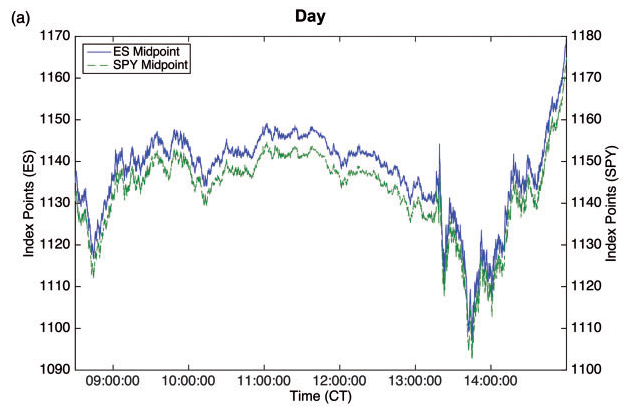
\includegraphics[scale=0.7]{pics/HTF_Corr_1}
\end{frame}


\begin{frame}[noframenumbering]{\citet*{budish_high-frequency_2015}}
	ES and SPY are the two largest instruments tracking SP500. In theory perfectly correlated. Panel (b) shows a trading hour.
	\center
	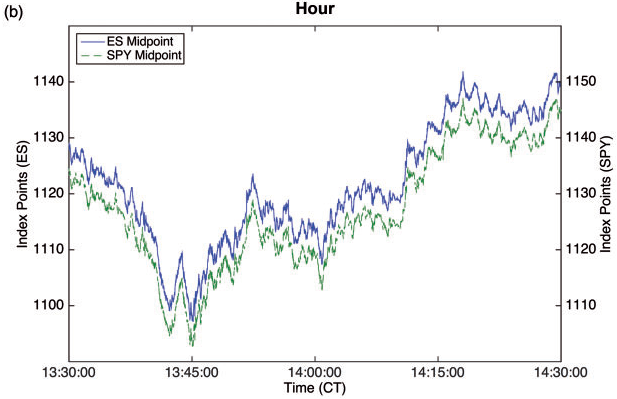
\includegraphics[scale=0.7]{pics/HTF_Corr_2}
\end{frame}


\begin{frame}[noframenumbering]{\citet*{budish_high-frequency_2015}}
	ES and SPY are the two largest instruments tracking SP500. In theory perfectly correlated. Panel (c) shows a trading minute.
	\center
	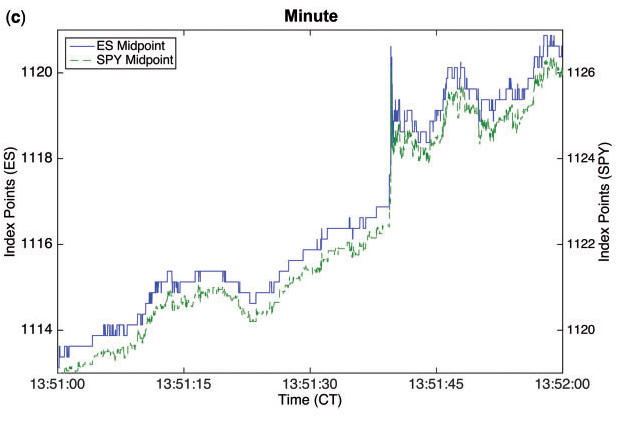
\includegraphics[scale=0.7]{pics/HTF_Corr_3}
\end{frame}


\begin{frame}[noframenumbering]{\citet*{budish_high-frequency_2015}}
	ES and SPY are the two largest instruments tracking SP500. In theory perfectly correlated. Panel (d) shows a high-frequency breakdown.
	\center
	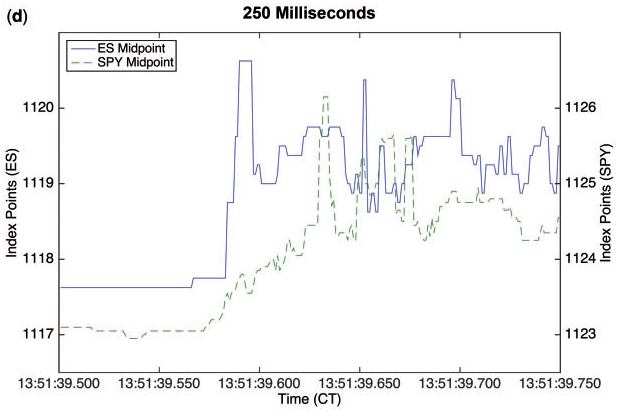
\includegraphics[scale=0.7]{pics/HTF_Corr_4}
\end{frame}


\begin{frame}[noframenumbering]{\citet*{budish_high-frequency_2015}}
	The figure below shows the correlation between ET and SPY by time interval for different years.
	\center
	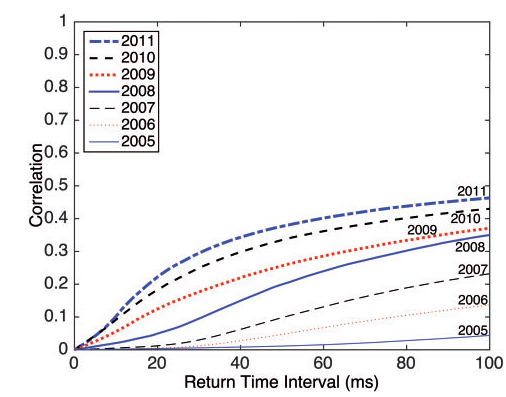
\includegraphics[scale=0.7]{pics/HTF_Corr_Time}
\end{frame}


\begin{frame}{\citet*{budish_high-frequency_2015}}
	The figure below shows median arbitrage profits over time. Very stable, total $\sim \$75$m/yr
	\center
	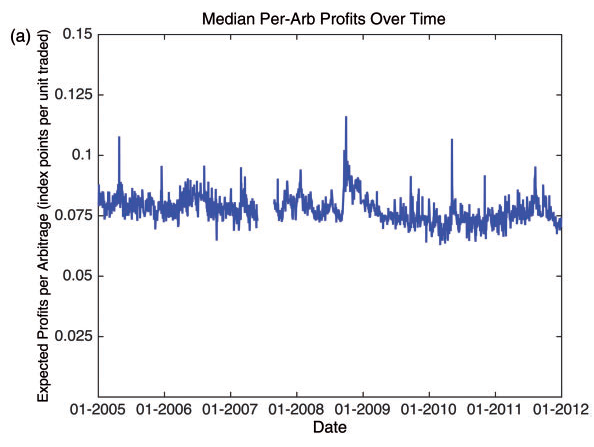
\includegraphics[scale=0.7]{pics/HTF_ArbitrageProfitsTime}
\end{frame}


\begin{frame}{Model of a continuous market}
	\structure{Security}
	\begin{itemize}
		\item \textbf{Value}: There is a signal $y$, which is perfectly correlated with the value $x$. Signal $y$ follows compound Poisson distribution.
		\item \textbf{Comp. Poisson}: Jumps arrive at rate $\lambda_{jump}$ and have size $J \sim F_{jump}$.
	\end{itemize}
	\structure{Players}
	\begin{itemize}
		\item \textbf{Noise traders}: arrive according to Poisson process ($\lambda_{invest}$)
		\begin{itemize}
			\item Want to buy/sell one unit
			\item Incur cost of delay, so use marketable limit orders $\simeq$ market orders
		\end{itemize}
		\item \textbf{HFTs}: There are $N$ HFT firms who use market or limit order
	\end{itemize}
	\structure{Order processing}
	\begin{itemize}
		\item If multiple orders/messages at same time, uniform random \\ draw to determine first to be processed
	\end{itemize}
\end{frame}


\begin{frame}{Equilibrium}
	\structure{Equilibrium properties}: Focus on equilibrium with the following properties
	\begin{itemize}
		\item \textbf{Endogenous market maker}: 1 HFT \textit{endogenously} takes the role of liquidity provider. Refer to this as the market maker (MM).
		\item \textbf{Adverse selection}: $N-1$ HFTs act as \textit{stale quote snipers}
	\end{itemize}
	\structure{Market maker}
	\begin{itemize}
		\item \textbf{Quotes}: Suppose signal is  $y$. Set $a=y+\frac{s}{2}$ and $b=y-\frac{s}{2}$ where $s$ is the spread.
		\item \textbf{News}: If news arrive and the new signal is $y'$, send message to cancel quotes $a$ and $b$ and post new ones: $a'=y'+\frac{s}{2}$ and $b'=y'-\frac{s}{2}$. Noise traders are slower at receiving news.
	\end{itemize}
	\structure{Snipers}
	\begin{itemize}
		\item Trade if $|y'-y|>\frac{s}{2}$.
	\end{itemize}
\end{frame}


\begin{frame}{Equilibrium (2)}
	\begin{itemize}
		\item \textbf{Market maker profits}: The MM \structure{flow profits} (per $dt$ period, normalized by $dt$) are
		\[
		\lambda_{invest}\cdot \frac{s}{2}-\lambda_{jump}\cdot \mathbb{P}\left(J>\frac{s}{2}\right) \cdot \mathbb{E} \left[J-\frac{s}{2} \mid J>\frac{s}{2}\right] \cdot \frac{N-1}{N}.
		\]
		\item \textbf{Sniper profits}: The profits to stale-quote snipers are
		\[
		\lambda_{jump}\cdot \mathbb{P} \left(J>\frac{s}{2} \right) \cdot \mathbb{E} \left[J-\frac{s}{2} \mid J>\frac{s}{2}\right] \cdot \frac{1}{N}.
		\]
		\item \textbf{Equilibrium condition}: Make HFT indifferent btw MM and sniper:
		\[
		\lambda_{invest} \cdot \frac{s}{2} = \lambda_{jump}\cdot \mathbb{P} \left(J>\frac{s}{2} \right) \cdot \mathbb{E} \left[J-\frac{s}{2} \mid J>\frac{s}{2}\right] .
		\]
		\item \textbf{Lack of competition}: Spread $s$ does not depend on $N$.
	\end{itemize}
\end{frame}


\begin{frame}{Continuous auction market versus batch}
	\begin{itemize}
		\item \textbf{Conclusion}: There will be a \structure{positive bid-ask spread} in continuous market (even as $N \rightarrow \infty)$, despite \alert{no asymmetric information} (kind of)
		\item \textbf{Market failure}: Authors argue that this failure is built into the market via processing mechanism
		\item \textbf{Proposed solution}: Frequent batch auction
		\begin{itemize}
			\item Auction every $\tau$ moments. Fast institutions have latency $\delta_{fast}$ and slow institutions latency $\delta_{slow}$. Three intervals:
			\begin{enumerate}
				\item  $[0,\tau-\delta_{slow}]$: all institutions trade, no AS
				\item  $[\tau-\delta_{slow},\tau-\delta_{fast}]$: only fast institutions trade, AS
				\item  $[\tau-\delta_{fast},\tau]$: no institution trade (inefficient)
			\end{enumerate}
		\end{itemize}
		\item \textbf{Outcome}: Before, fast trader always has advantage; now only $\frac{\delta}{\tau}$ of the time, where $\delta = \delta_{slow}-\delta_{fast}$. If $\delta=$ 100 microseconds and $\tau=$ 100 milliseconds. Then $\frac{\delta}{\tau}=\frac{1}{1000}$. Large reduction in HFT importance.
	\end{itemize}
\end{frame}


\begin{frame}{BCS Conclusion}
	\begin{itemize}
		\item By design, continuous trading generates arbitrage opportunities
		\item Firms overinvest in speed in attempts to reap these arbitrage profits
		\item Risk of being sniped contributes to the spread
		\item Use better market design (frequent auctions) to improve this
	\end{itemize}
\end{frame}



\section{Blockchain and cryptocurrencies}

\begin{frame}{Blockchain and cryptocurrencies}
	\begin{itemize}
		\item Our discussion would be incomplete without mentioning \alert{blockchain} and \alert{cryptocurrencies}, the biggest trend of 2017
		\begin{itemize}
			\item blockchain is a ``distributed ledger'' technology
			\item crypto uses blockchain to record transactions in some tokens
		\end{itemize}
		\item In addition to below, you can find some economic discussion of crypto in \citet*{nica_cryptocurrencies_2017}
	\end{itemize}
\end{frame}


\begin{frame}{How should it work?}
	\begin{itemize}
		\item Cryptos (bitcoin, ethereum) are like distributed payment systems
		\item You can translate that to a financial market:
		\begin{itemize}
			\item Say coins serve as shares of some company
			\item Or there is a decentralized exchange that records stock ownership transactions in a blockchain
		\end{itemize}
	\end{itemize}
\end{frame}


\begin{frame}{Why the hype?}
	%Perceived benefits of blockchain/crypto-based markets:
	\begin{itemize}
		\item \structure{Decentralization}: no exchange to profit from traders $\Rightarrow$ lower order costs
		\item \structure{Transparency}: transaction history is visible, order flow is visible, counterparty's trading history visible
		\begin{itemize}
			\item note: there is very little anonymity, contrary to what some say!
		\end{itemize}
		\item \structure{Smart contracts}: algotrading by design
	\end{itemize}
\end{frame}


\begin{frame}[label=problems]{Why not?}
	\begin{itemize}
		\item \alert{Limited processing capacity}: block size and frequency is $\approx$fixed
		\begin{itemize}
			\item Visa: 150m tx/day; Bitcoin (15.02.21): 300k tx/day
		\end{itemize}
		\item \alert{Order costs} and \alert{execution risk}: you have to bid for your transaction to be accepted into a block.
		\begin{itemize}
			\item This is on top of execution risk from other sources (for limit orders)
			\item Average order costs fluctuate over time \hyperlink{bcfee}{\beamerbutton{graph}}
			\item There are concerns that miners inflate fees (\cite{lehar_miner_2020})
		\end{itemize}
		\item \alert{Delay}: blocks are only processed rarely (one per 10 min avg for bitcoin) \hyperlink{blocktime}{\beamerbutton{graph}}
		\item \alert{Clearing and settlement}: without a trusted mediator, counterparty risk instensifies
		\item \alert{No transparency requirements}: it is more difficult to enforce \\ disclosure of financial info from firms
	\end{itemize}
\end{frame}


\begin{frame}{Crypto: Conclusion}
	\begin{itemize}
		\item generally cool and good
		\item crypto and blockchain have potential, but they are not a panacea
	\end{itemize}
\end{frame}



\appendix
\begin{frame}<handout:0>[allowframebreaks]{References}
	\bibliography{../teaching}
	\bibliographystyle{abbrvnat}
\end{frame}


\begin{frame}<handout:0>[label=bcfee]
	\centering
	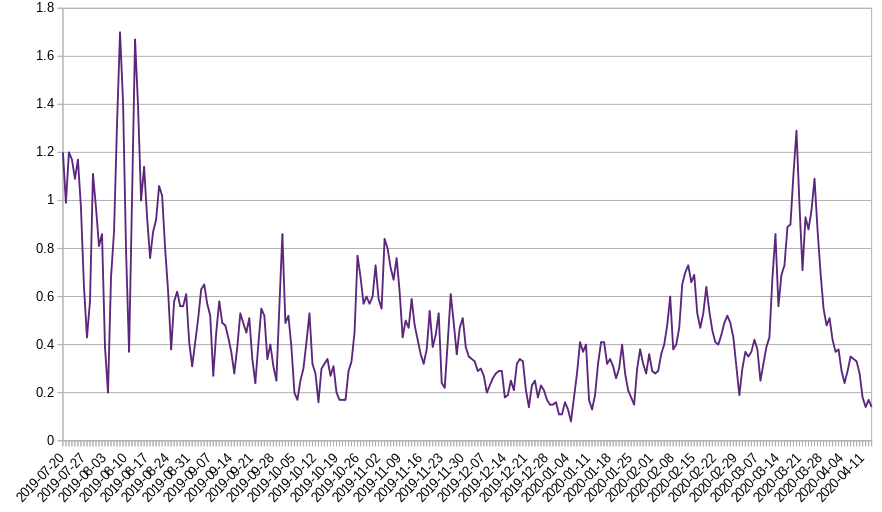
\includegraphics[width=0.8\paperwidth]{pics/bitcoin_orderfee}
	
	Bitcoin avg daily order processing fee, USD per transaction \hyperlink{problems}{\beamerbutton{back}}
\end{frame}


\begin{frame}<handout:0>[label=blocktime]
	\centering
	\includegraphics[width=0.7\paperwidth]{pics/blocktime}
	
	Histogram of time between blocks (\cite{lehar_miner_2020}) \hyperlink{problems}{\beamerbutton{back}}
\end{frame}

\end{document} 